% begin module rates-physics-ex1
\begin{frame}[t]
\begin{example}[Example 1, p. 171]
The position of a particle is given by the equation
\abovedisplayskip=0pt
\belowdisplayskip=0pt
\[
s = f(t) = t^3 - 6t^2 + 9t
\]
where $t$ is measured in seconds and $s$ in meters.
\begin{enumerate}
\item  Find the velocity at time $t$.
\item  What is the velocity after 2 s? After 4 s?
\item  When is the particle at rest?
\item  When is the particle moving forward? 
\item  Find the acceleration at time $t$ and after 4 s.
\item  Graph the position, velocity, and acceleration functions.
\item  When is the particle speeding up?  When is it slowing down?
\end{enumerate}
\end{example}
\end{frame}


\begin{frame}[t]
\begin{example}[Example 1, p. 171]
The position of a particle is given by the equation
\abovedisplayskip=0pt
\belowdisplayskip=0pt
\[
s = f(t) = t^3 - 6t^2 + 9t
\]
where $t$ is measured in seconds and $s$ in meters.
\begin{enumerate}
\item<1-| alert@2-3>  Find the velocity at time $t$.
\item<1-| alert@4->  What is the velocity after 2 s? After 4 s?
\end{enumerate}
\begin{enumerate}
\item<2->  The velocity function is the derivative of the position function.
\[
\uncover<2->{%
v(t) = \frac{\diff s}{\diff t} =%
}%
\uncover<3->{%
3t^2 - 12 t + 9.
}%
\]
\item<4->  \alert<handout:0| 4-5>{$v(2) = 3(2)^2 - 12(2) + 9 = \uncover<5->{12-24+9 = -3}$ \uncover<5->{m/s.}}  \uncover<6->{\alert<handout:0| 6-7>{$v(4) = 3(4^2) - 12(4) + 9 =\uncover<7->{ 48 - 48 + 9 = 9}$ \uncover<7->{m/s.}}}
\end{enumerate}
\end{example}
\end{frame}


\begin{frame}[t]
\begin{example}[Example 1, p. 171]
The position of a particle is given by the equation
\abovedisplayskip=0pt
\belowdisplayskip=0pt
\[
s = f(t) = t^3 - 6t^2 + 9t
\]
where $t$ is measured in seconds and $s$ in meters.
\begin{enumerate}
\setcounter{enumi}{2}
\item<1-| alert@2-4>  When is the particle at rest?
\item<1-| alert@5->  When is the particle moving forward? 
\end{enumerate}
\begin{enumerate}
\setcounter{enumi}{2}
\item<2->  The particle is at rest when $v = 0$.
\abovedisplayskip=0pt
\belowdisplayskip=0pt
\begin{eqnarray*}
\uncover<2->{%
v(t)%
}%
& \uncover<2->{ = } &%
\uncover<2->{%
0%
}\\%
\uncover<2->{%
3t^2 - 12 t + 9%
}%
& \uncover<2->{ = } &%
\uncover<2->{%
0%
}\\%
\uncover<3->{%
3(t - 1)(t - 3)%
}%
& \uncover<3->{ = } &%
\uncover<3->{%
0%
}\\%
\uncover<4->{%
t%
}%
& \uncover<4->{ = } &%
\uncover<4->{%
1 \textrm{ or } 3%
}\\%
\end{eqnarray*}
\vspace{-.4in}
\item<5->  The particle moves forward when $v > 0$; that is, when $3(t-1)(t-3) > 0$.  This happens when both factors are positive $(t > 3)$ or both are negative $(t < 1)$.
\end{enumerate}
\end{example}
\end{frame}


\begin{frame}[t]
\begin{example}[Example 1, p. 171]
The position of a particle is given by the equation
\abovedisplayskip=0pt
\belowdisplayskip=0pt
\[
s = f(t) = t^3 - 6t^2 + 9t
\]
where $t$ is measured in seconds and $s$ in meters.
\begin{enumerate}
\setcounter{enumi}{4}
\item<1-| alert@2-5>  Find the acceleration at time $t$ and after 4 s.
\item<1-| alert@6->  Graph the position, velocity, and acceleration functions. 
\end{enumerate}
\begin{enumerate}
\setcounter{enumi}{4}
\item<2->  The acceleration function is the derivative of the velocity function.
\[
\uncover<2->{%
a(t) = \frac{\diff \alert<handout:0| 3>{v}}{\diff t} = %
}%
\uncover<3->{%
\frac{\diff}{\diff t} (\alert<handout:0| 3>{3t^2-12t + 9}) = %
}%
\uncover<4->{%
6t - 12.
}%
\]
\uncover<5->{%
Then $a(4) = 6(4) - 12 = 12$ m/s$^2$.
}%
\item<6->  
\begin{center}
\ \uncover<6->{%
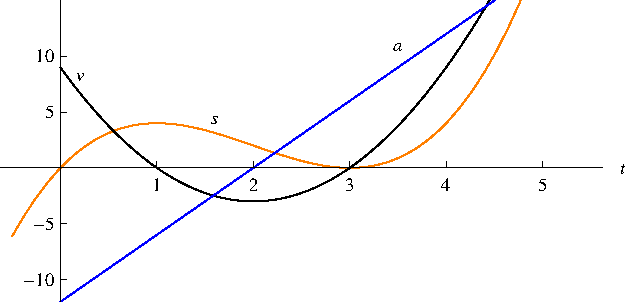
\includegraphics[height=2.5cm]{rates-of-change/pictures/03-07-ex1a.pdf}%
}%
\end{center}
\end{enumerate}
\end{example}
\end{frame}



\begin{frame}[t]
\begin{example}[Example 1, p. 171]
The position of a particle is given by the equation
\abovedisplayskip=0pt
\belowdisplayskip=0pt
\[
s = f(t) = t^3 - 6t^2 + 9t
\]
where $t$ is measured in seconds and $s$ in meters.
\begin{enumerate}
\setcounter{enumi}{6}
\item  When is the particle speeding up?  When is it slowing down?
\end{enumerate}
\begin{center}
\ \only<-3,6>{%
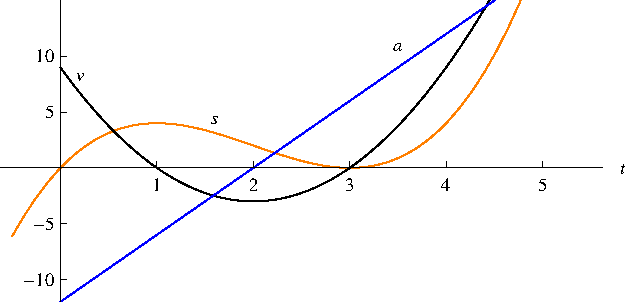
\includegraphics[height=2.5cm]{rates-of-change/pictures/03-07-ex1a.pdf}%
}%
\only<handout:0| 4>{%
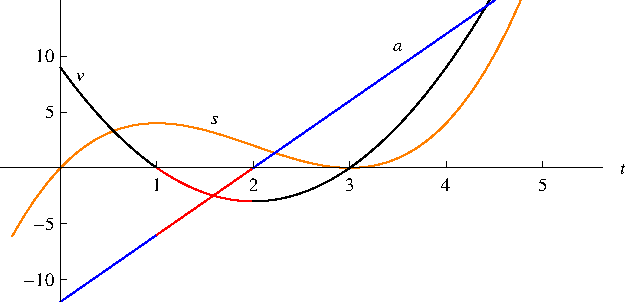
\includegraphics[height=2.5cm]{rates-of-change/pictures/03-07-ex1b.pdf}%
}%
\only<handout:0| 5>{%
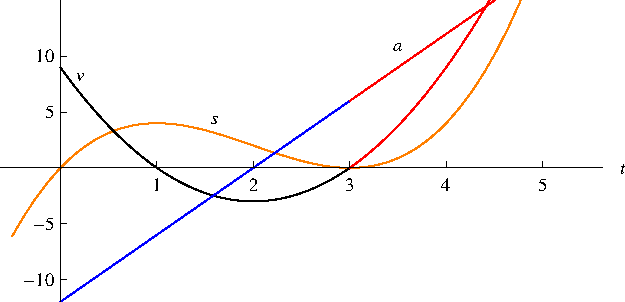
\includegraphics[height=2.5cm]{rates-of-change/pictures/03-07-ex1c.pdf}%
}%
\only<handout:0| 7>{%
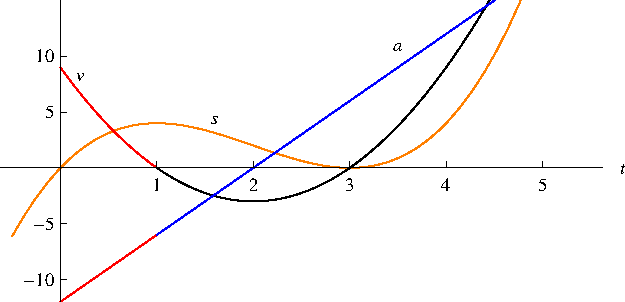
\includegraphics[height=2.5cm]{rates-of-change/pictures/03-07-ex1d.pdf}%
}%
\only<handout:0| 8>{%
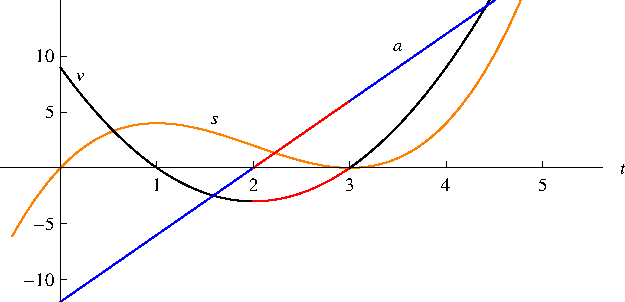
\includegraphics[height=2.5cm]{rates-of-change/pictures/03-07-ex1e.pdf}%
}%
\end{center}
\vspace{-.3in}
\begin{enumerate}
\setcounter{enumi}{6}
\item<2->  The particle is speeding up when $v$ and $a$ are both positive or both negative.

\uncover<3->{%
This happens when $\alert<handout:0| 4>{1 < t < 2}$ and when $\alert<handout:0| 5>{t > 3}$.
}%

\uncover<6->{%
It is slowing down when $v$ and $a$ have opposite signs.  This happens when $\alert<handout:0| 7>{0\leq t < 1}$ and $\alert<handout:0| 8>{2 < t < 3}$.
}%
\end{enumerate}
\end{example}
\end{frame}
% end module rates-physics-ex1
